% \section{Preliminary Results}
% The dynamic system modelling framework has been implemented and validated.
% An automotive fuel cell system presented by Pukrushpan \etal \cite{pukrushpanControlFuelCell2004a} was chosen as a validation case due to the availability the source code to the authors and the simple, well documented component models. Following the implementation of said component models, the response of the system to a prescribed stack current profile was evaluated, and compared to the response of the original models. The time-series output of the stack voltage is given in Figure \ref{fig:ts} and a calibration plot is given in Figure \ref{fig:cal}.
% \medskip
% \noindent
% \begin{minipage}[t]{\linewidth}
% 	\begin{center}
% 		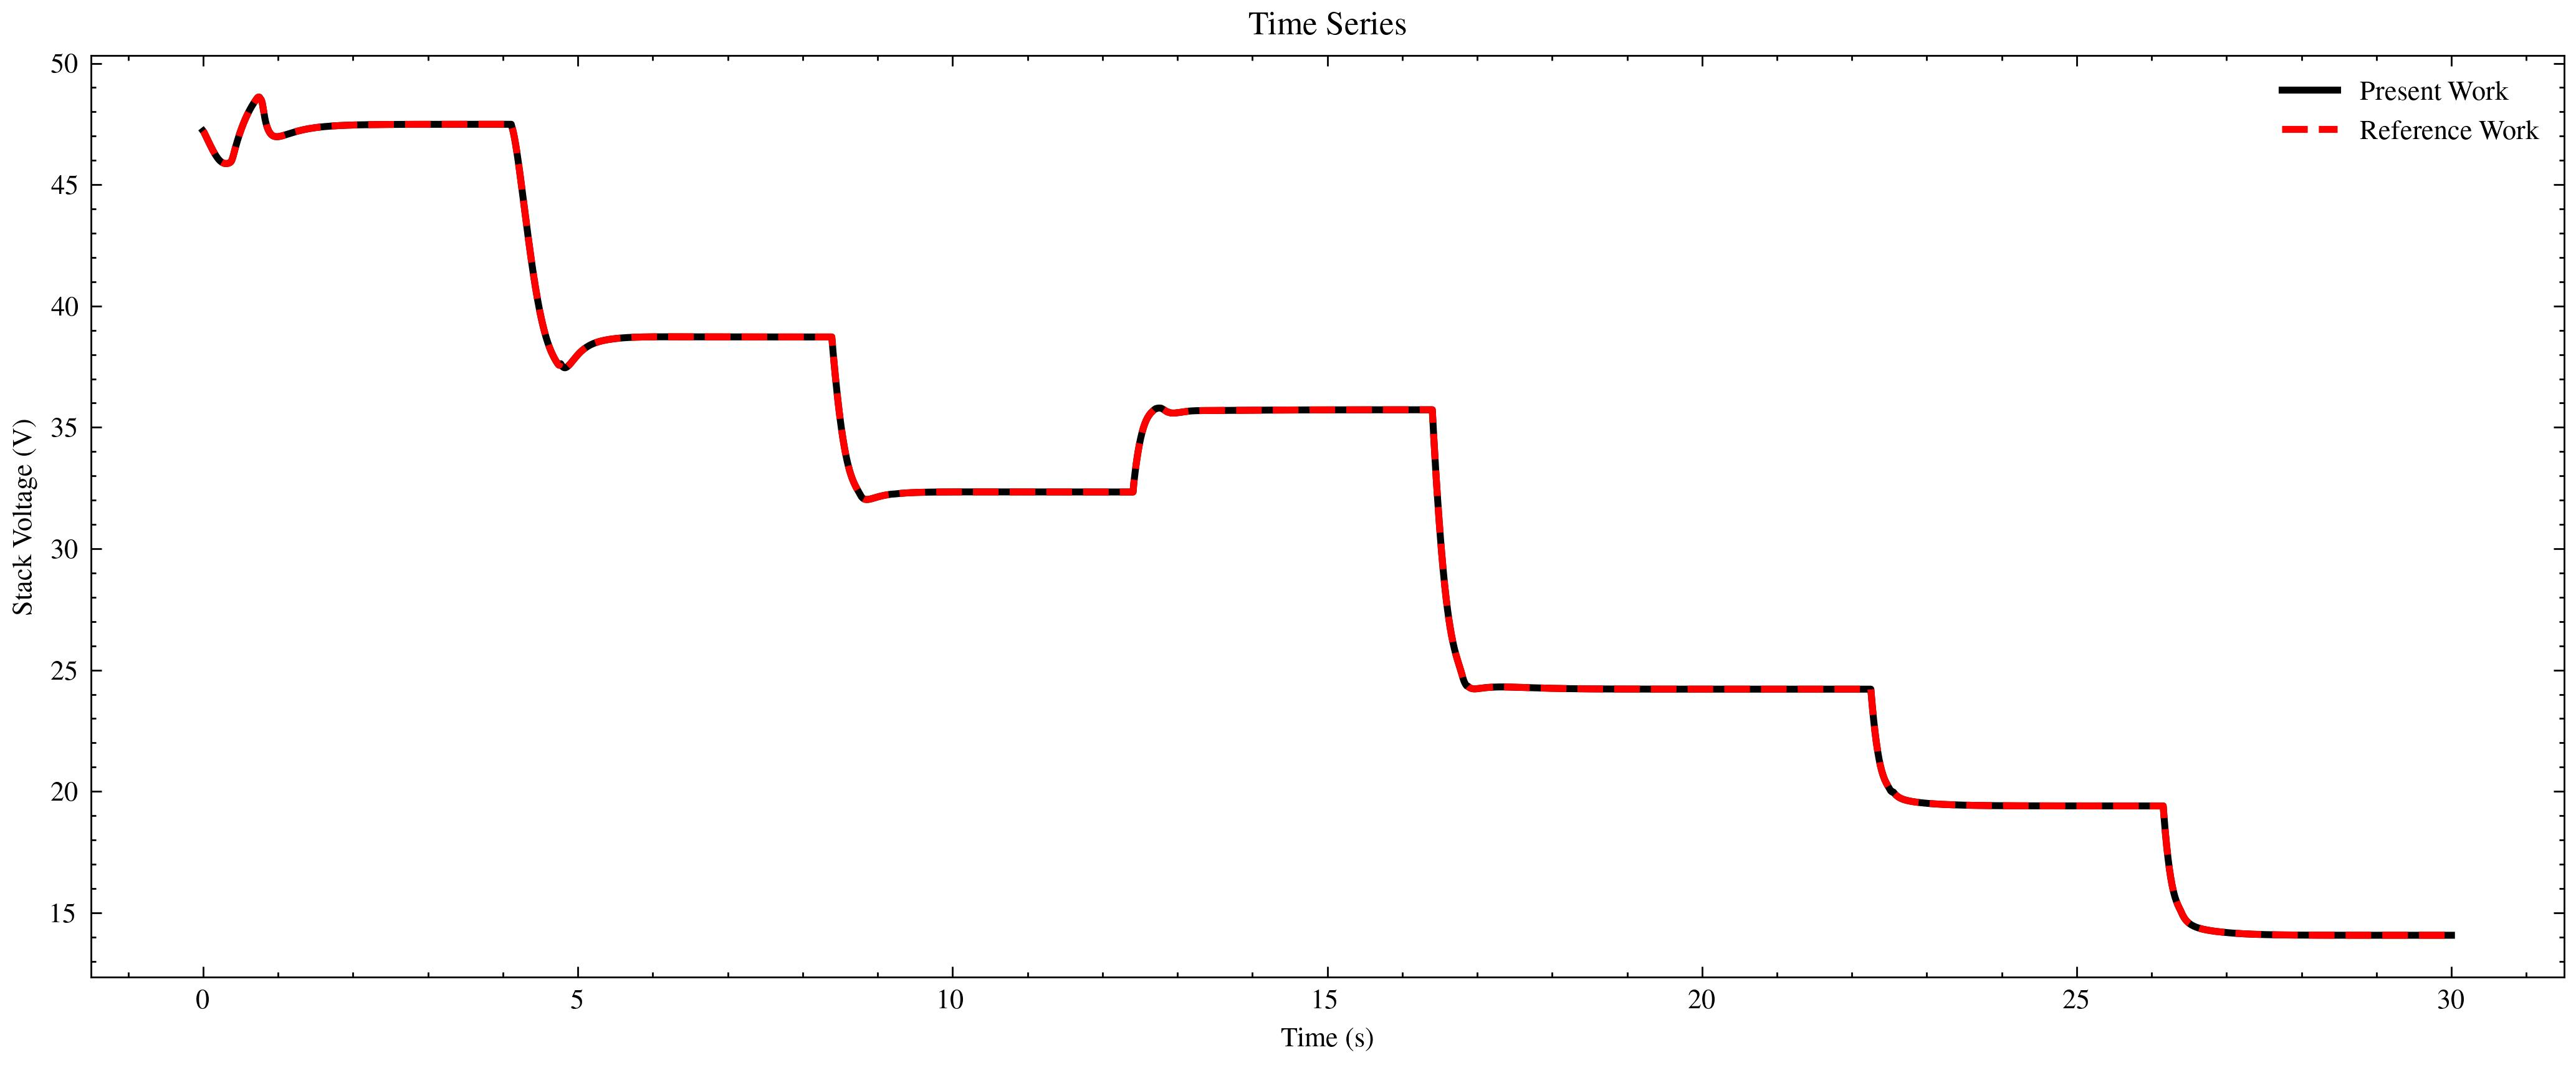
\includegraphics[height=18em]{figures/voltage_ts.jpg}
% 		\captionof{figure}{Some caption}
% 		\label{fig:ts}
% 	\end{center}
% \end{minipage}%
% \hfill\vspace{1em}
% \begin{minipage}[t]{\linewidth}
% 	\begin{center}
% 		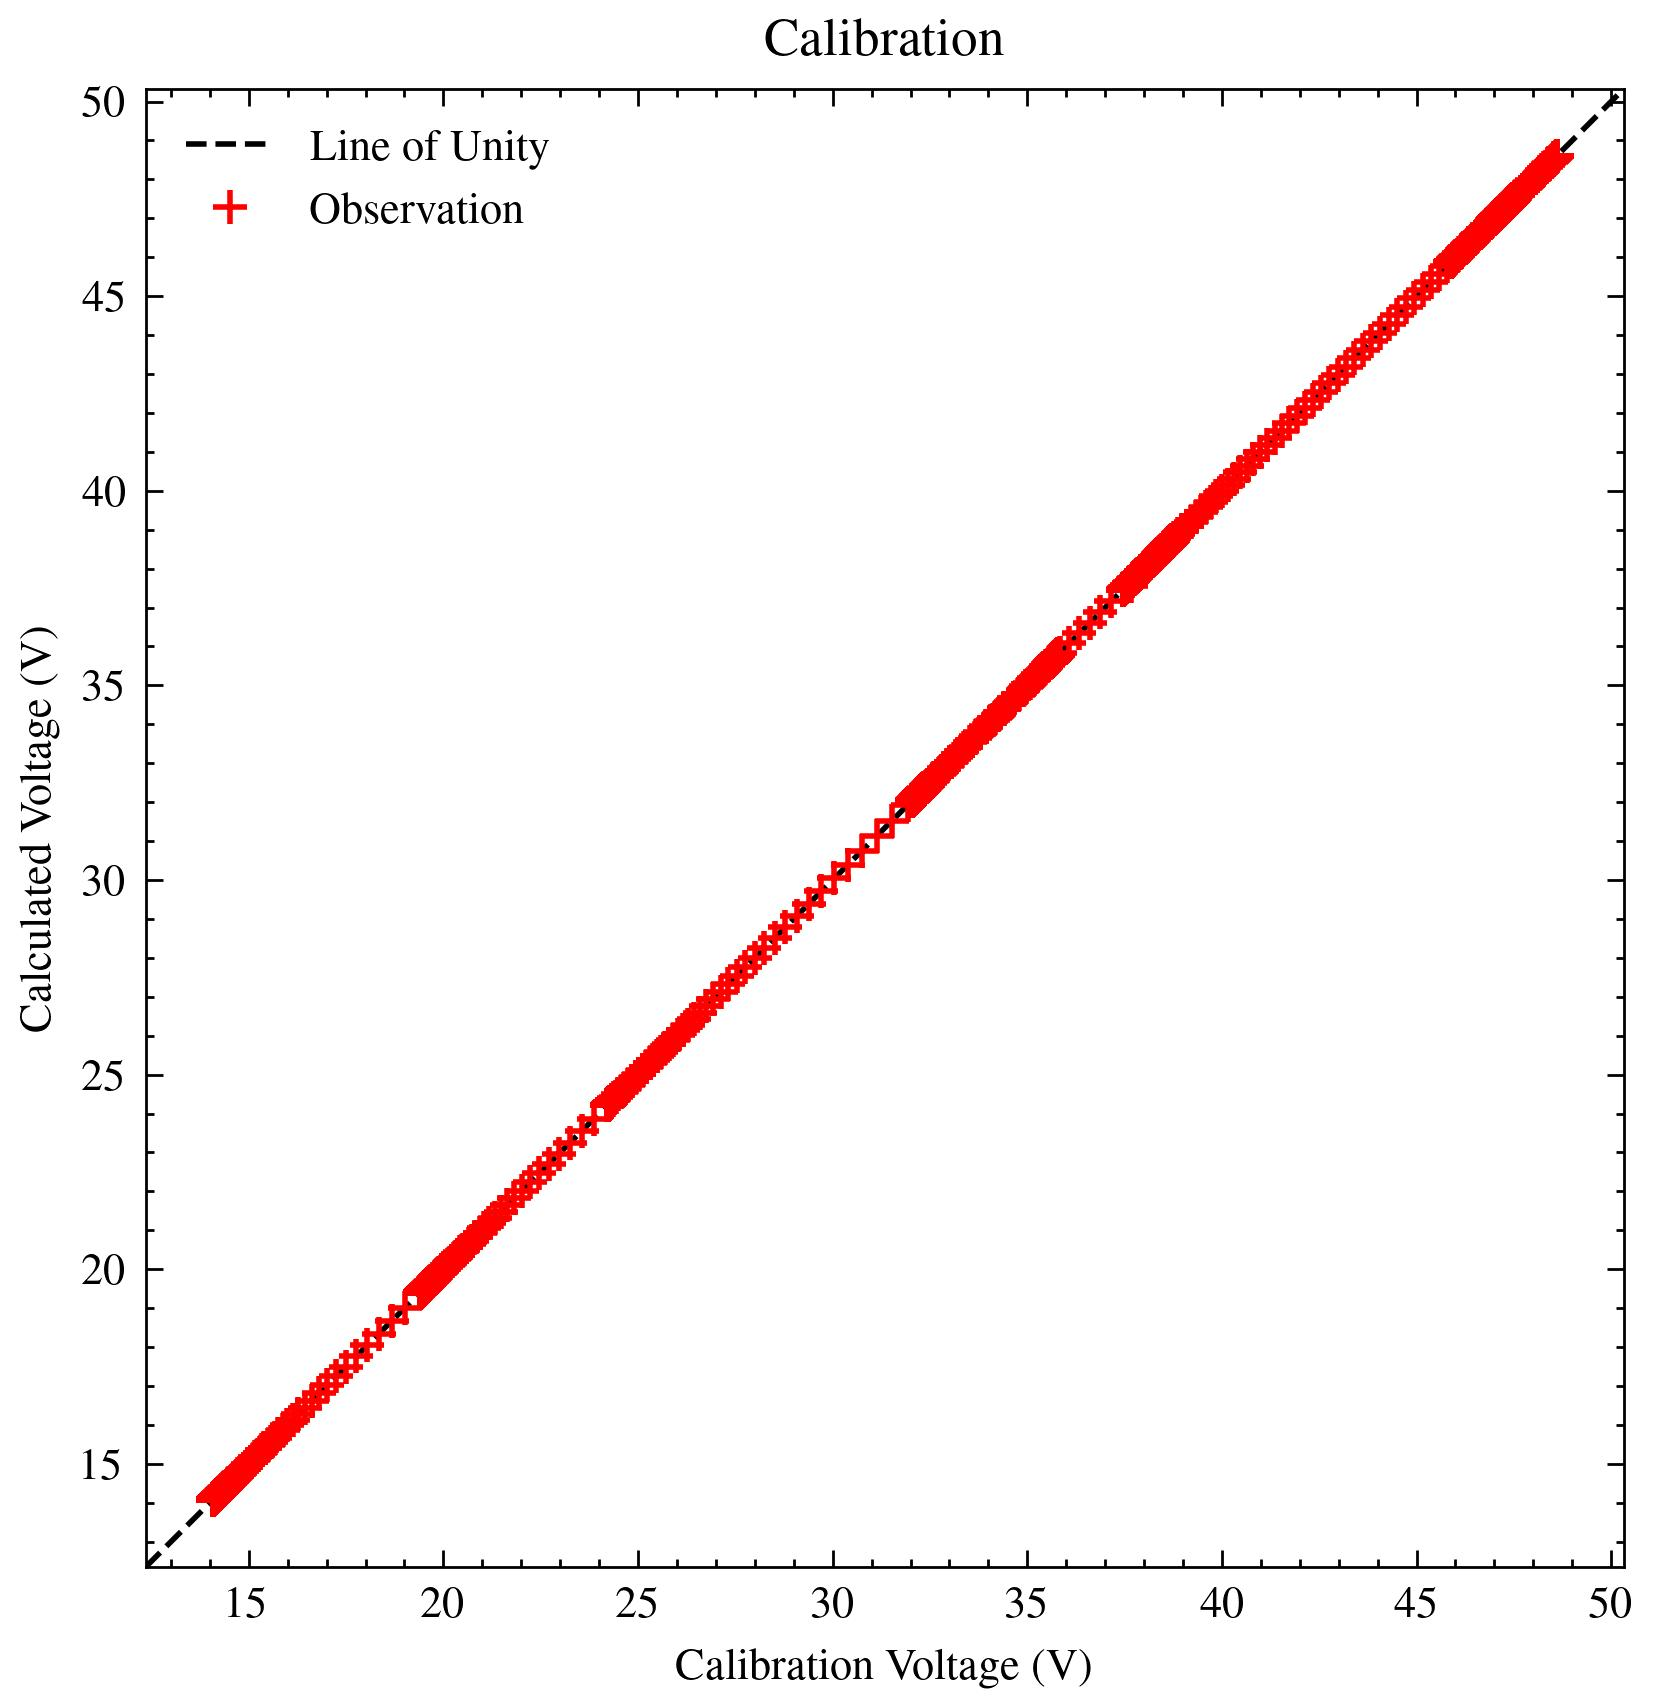
\includegraphics[height=18em]{figures/voltage_cal.jpg}
% 		\captionof{figure}{Some caption}
% 		\label{fig:cal}
% 	\end{center}
% \end{minipage}
